% CESC 410L lab report.
%
% NOTE TO WHOEVER EDITS THIS: keep this file free of references to any
% tooling, scripts or repository paths. It is a submitted document. Build and
% packaging instructions belong in reference_docs/report_guide.md, not here.
% Comment-only lines are stripped at package time as a backstop, but do not
% rely on that.
%
% DELIBERATE EXCEPTION: a lab report keeps its OWN preamble and does not
% \input the shared coursework preamble the homework solutions use. Three
% reasons, in order of weight:
%   1. A handed-in .tex has to compile wherever the reader puts it. A shared
%      preamble is reached by a relative path that resolves only at one exact
%      depth inside this repository, so the submitted copy would not build.
%   2. The packaging check rejects a repository path on a non-comment line,
%      and an \input of the course macros file is exactly that.
%   3. A report is prose plus figures under a title block. It wants no running
%      head, no answer box and no problem header -- which is most of what the
%      shared preamble exists to provide. It also needs listings, which the
%      shared preamble does not load.
% The overlap is four package lines, a margin and a captionsetup. That is the
% whole price, and it buys a document that stands on its own anywhere.

\documentclass[11pt]{article}

\usepackage[margin=1in]{geometry}
\usepackage{amsmath, amssymb}     % equations
\usepackage{graphicx}             % \includegraphics
\usepackage{booktabs}             % clean tables
\usepackage{listings}             % code snippets
\usepackage{xcolor}
\usepackage[colorlinks=true, allcolors=blue]{hyperref}
\usepackage{caption}

% Look for figures beside this file first, then one level up. The second entry
% lets a copy of this document sitting in a subfolder still find figs/.
\graphicspath{{./}{../}}

% Code style: Courier New equivalent at 10pt, per the CEC 320 template's
% "code in Courier New 12, single spacing". Light background, no dark blocks --
% reports may be printed.
\lstset{
  basicstyle=\ttfamily\small,
  breaklines=true,
  frame=single,
  backgroundcolor=\color{gray!8},
  showstringspaces=false,
  captionpos=b,
  language=Python,
}

\title{CESC 410L --- Lab 1: Artifact Collection}
\author{Gatlin Nelson \\ Section 01}
\date{Fall 2026}

\usepackage{float}
\begin{document}
\maketitle

This document collects the artifacts the three Lab 1 tasks call for, in the order
the handout lists them.

%======================================================================
\section*{Project Management Task}
%======================================================================

\subsection*{Artifact 1 --- output of \texttt{dsp26 -{}-help}}

\begin{lstlisting}
 Usage: dsp26 [OPTIONS] COMMAND [ARGS]...

 Commands
   plot-sinusoids-td-fd   Plot time-domain waveform and frequency-domain
                          spectrum of sinusoids.
   play-plot-audio        Play and plot audio signal.
                          Use --path-name to load audio file from.
\end{lstlisting}

\subsection*{Artifact 2 --- the Audio Player window}

\begin{figure}[H]
  \centering
  \IfFileExists{figs_player/audio_player_window.png}
    {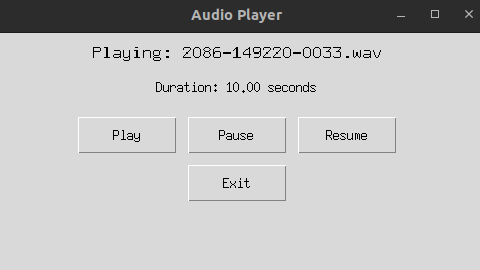
\includegraphics[width=0.6\textwidth]{figs_player/audio_player_window.png}}
    {\fbox{\parbox[c][0.25\textwidth][c]{0.75\textwidth}{\centering\itshape
       Screenshot to be captured from the running application.}}}
  \caption{The Audio Player window shown while the audio file plays.}
\end{figure}

\subsection*{Properties reported for the supplied file}

The command prints the WAV header fields before drawing anything:

\begin{lstlisting}
Number of channels: 1
Sample width (bytes): 2
Frame rate (sample rate): 16000
Number of frames: 160000
Duration (seconds): 10.0
\end{lstlisting}

One channel of 16-bit samples at 16\,kHz, and
$160000 / 16000 = 10.0$\,s. The content is two constant-amplitude sinusoids at
440\,Hz and 554\,Hz, which is what the five figures below show.

\subsection*{Artifacts 3--7 --- the five figures}

\begin{figure}[H]
  \centering
  \includegraphics[width=0.62\textwidth]{figs/lab1_audio_fig1_waveform_full.png}
  \caption{Handout Figure 1 --- waveform of the whole file, 0 to 10\,s. It fills as a
           solid block between $\pm 1.0$ because the signal is a sustained tone
           of constant amplitude: there is no onset, no decay and no silence
           anywhere in the file for the envelope to show.}
\end{figure}

\begin{figure}[H]
  \centering
  \includegraphics[width=0.62\textwidth]{figs/lab1_audio_fig2_waveform_zoom.png}
  \caption{Handout Figure 2 --- waveform zoomed to 0.4--1.4\,s. The zoom resolves what
           Figure 1 could not: the two tones interfere, and their sum swells
           and collapses at their difference frequency,
           $554.4 - 440.0 = 114.4$\,Hz. The window is one second wide and
           contains 114 such lobes.}
\end{figure}

\begin{figure}[H]
  \centering
  \includegraphics[width=0.62\textwidth]{figs/lab1_audio_fig3_spec_linear.png}
  \caption{Handout Figure 3 --- spectrogram, linear frequency axis. All of the energy
           lies in one band near the bottom of the 0--8\,kHz range and the plot
           is empty above roughly 1\,kHz. On this axis the two tones are
           114\,Hz apart out of 8000 and cannot be told apart.}
\end{figure}

\begin{figure}[H]
  \centering
  \includegraphics[width=0.62\textwidth]{figs/lab1_audio_fig4_spec_log.png}
  \caption{Handout Figure 4 --- spectrogram, logarithmic frequency axis. The same data
           as Figure 3, but the expanded low end separates the band into the
           two distinct horizontal lines it is made of, either side of the
           512\,Hz tick. Both run flat for the full ten seconds, with no
           harmonics above them.}
\end{figure}

\begin{figure}[H]
  \centering
  \includegraphics[width=0.62\textwidth]{figs/lab1_audio_fig5_spec_mel.png}
  \caption{Handout Figure 5 --- spectrogram, mel frequency axis. The mel scale is
           near-linear below 1\,kHz, so the two tones stay close together and
           the plot is black above about 512\,Hz --- the warping that helps
           with speech has little to work with on a signal this sparse.}
\end{figure}

\clearpage
%======================================================================
\section*{Experimental Task}
%======================================================================

A ten-second excerpt of music, converted to a single channel at a 16\,kHz
sample rate. The properties reported by the application confirm the format:

\begin{lstlisting}
Number of channels: 1
Sample width (bytes): 2
Frame rate (sample rate): 16000
Number of frames: 160000
Duration (seconds): 10.0
\end{lstlisting}

\begin{figure}[H]
  \centering
  \includegraphics[width=0.62\textwidth]{figs_music/lab1_audio_fig2_waveform_zoom.png}
  \caption{The second (zoomed-in) waveform figure, for the music file.}
\end{figure}

\begin{figure}[H]
  \centering
  \includegraphics[width=0.62\textwidth]{figs_music/lab1_audio_fig5_spec_mel.png}
  \caption{The last spectrum figure, for the music file.}
\end{figure}

\clearpage
%======================================================================
\section*{Programming Task}
%======================================================================

\subsection*{Code snippet}

\begin{lstlisting}[caption={\texttt{app\_cli.py} --- the two new options}]
    start_s: float = typer.Option(
        0.0, "--start-s",
        help="Start time in seconds for the zoomed waveform figure."),
    end_s: float = typer.Option(
        None, "--end-s",
        help="End time in seconds for the zoomed waveform figure."),
\end{lstlisting}

\begin{lstlisting}[caption={\texttt{recipes.py} --- passing them through}]
if start_s == 0.0 and end_s is None:
    zoom_start, zoom_end = HANDOUT_ZOOM_S      # (0.4, 1.4)
else:
    zoom_start, zoom_end = start_s, end_s

fig2 = plot_audio_sig_in_td(audio, sample_rate, zoom_start, zoom_end)
\end{lstlisting}

\subsection*{Code explanation}

Each \texttt{typer.Option} binds a Python parameter to a command-line flag. The
first argument is the value used when the flag is absent, the second is the
flag's spelling, and the annotated type drives both conversion and validation
--- so \texttt{-{}-start-s 0.5} arrives as the float \texttt{0.5}, and a
non-numeric value is rejected before any code runs. The help strings become the
text shown by \texttt{-{}-help}.

The defaults are those of \texttt{plot\_audio\_sig\_in\_td} itself, as the task
requires: zero, and ``to the end of the file''. Since that pair means the whole
file, supplying neither would make the zoomed figure a duplicate of the
full-waveform figure, so when neither is given the handout's own 0.4--1.4\,s
window is used instead; any explicit window is passed through unchanged.

No plotting code was modified. \texttt{plot\_audio\_sig\_in\_td} already
accepted an arbitrary window, so the task was to expose that capability at the
command line, not to implement it.

\begin{figure}[H]
  \centering
  \includegraphics[width=0.62\textwidth]{figs_music/lab1_audio_prog_zoom_0.5_1.5.png}
  \caption{The music file, zoomed from 0.5 to 1.5 seconds, produced with
           \texttt{-{}-start-s 0.5 -{}-end-s 1.5}.}
\end{figure}

\end{document}
